\vspace{-1mm}
\section{How Do Languages Benefit or Interfere with Each Other?}
\label{sec:lang-transfer}
\vspace{-1mm}

\textbf{Research Question:} \emph{Which languages synergize or interfere most with one another's performance?}

\begin{figure*}[htbp]
    \centering
    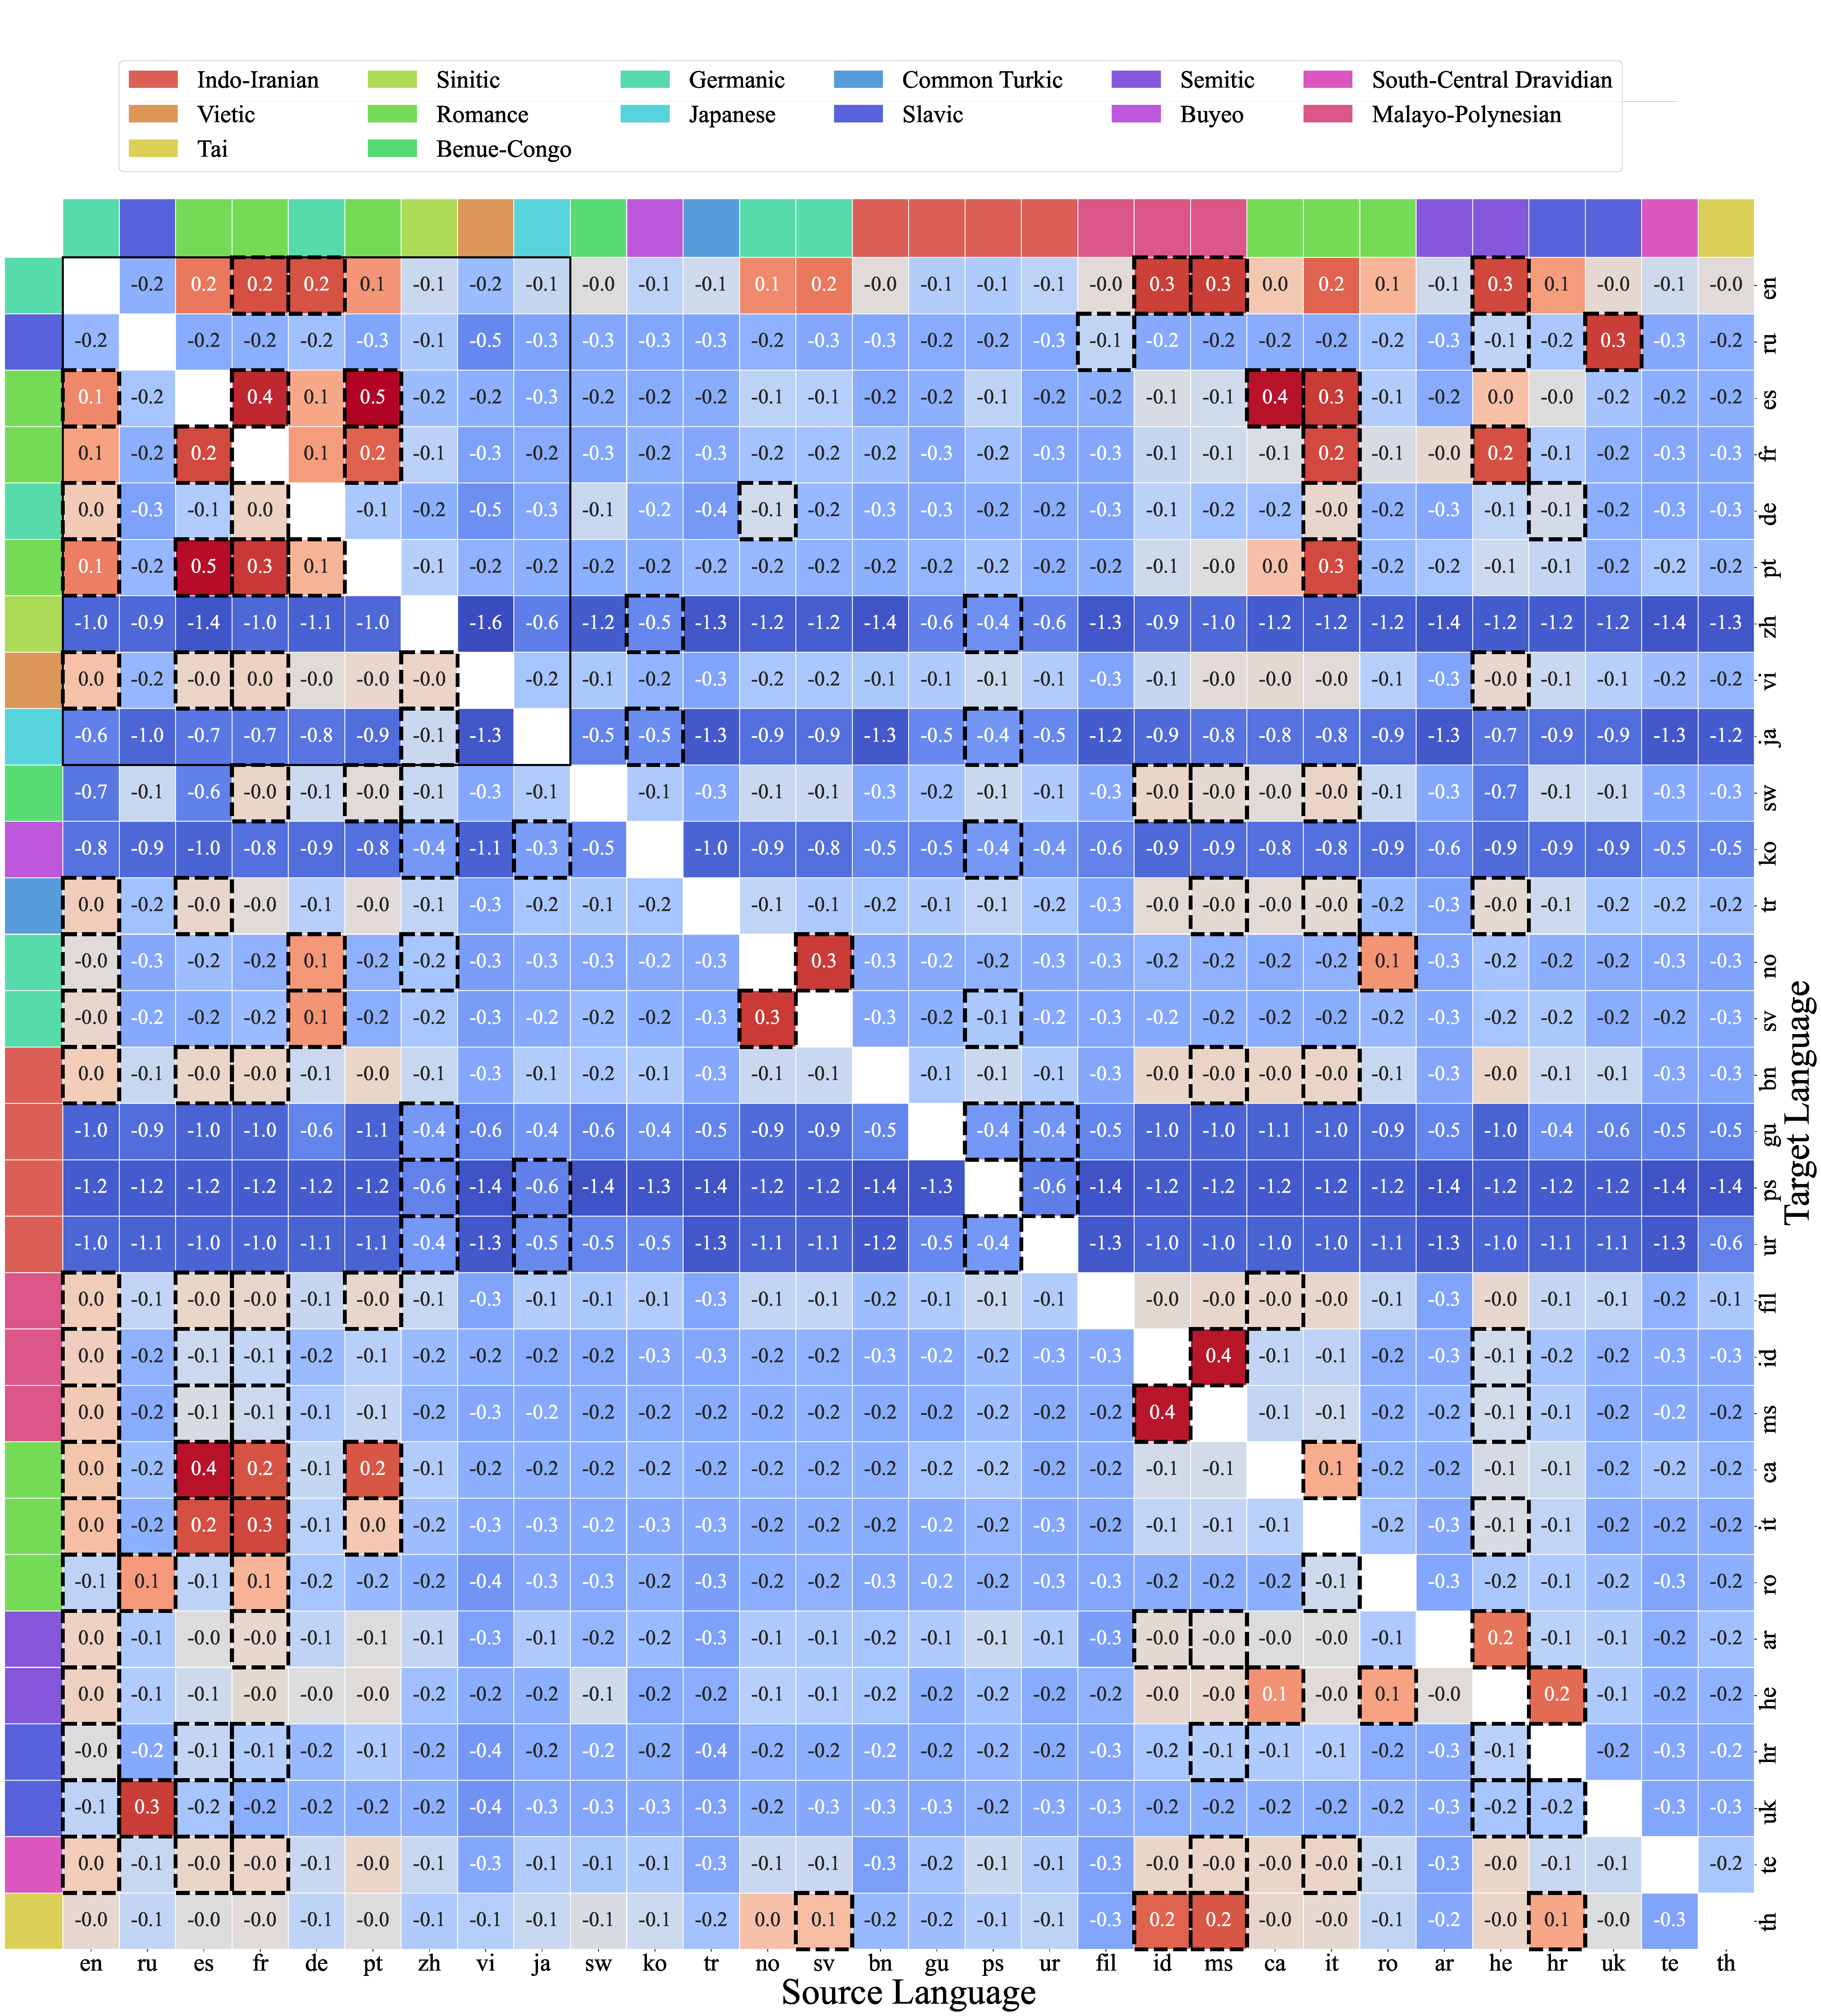
\includegraphics[width=0.85\textwidth]{figures/language-transfer/multilingual_heatmap_smaller.pdf}
    % \vspace{-3mm}
    \caption{
    The \textsc{Cross-Lingual Transfer Matrix}, depicting the measured Language Transfer Score across $30 \times 30$ language pairs.
    Positive scores indicate more positive transfer, negative scores more interference, during bilingual co-training.
    % the benefit/interference to the target language by (co-)training with the source language.
    The dashed boxes indicate the top-5 source languages for each target language.
    % We place a dashed box on the top-5 source languages for each target language.
    % The top left 9x9 are the \bts{} computed directly, whereas the rest are estimated from the \fas{}. 
    Refer to Appendix \ref{app:lang-transfer-bts-estimation} for full details, and \Cref{fig:language-transfer-heatmap-full} for the larger $38 \times 38$ matrix.
    \textbf{While English is the best source language for many of the languages, we find language similarity is highly predictive of these scores.} 
    }
    \label{fig:language-transfer-heatmap}
    % \vspace{-3mm}
\end{figure*}


\begin{figure}[htbp]
    \centering
    \begin{subfigure}[b]{0.45\textwidth}
        \centering
        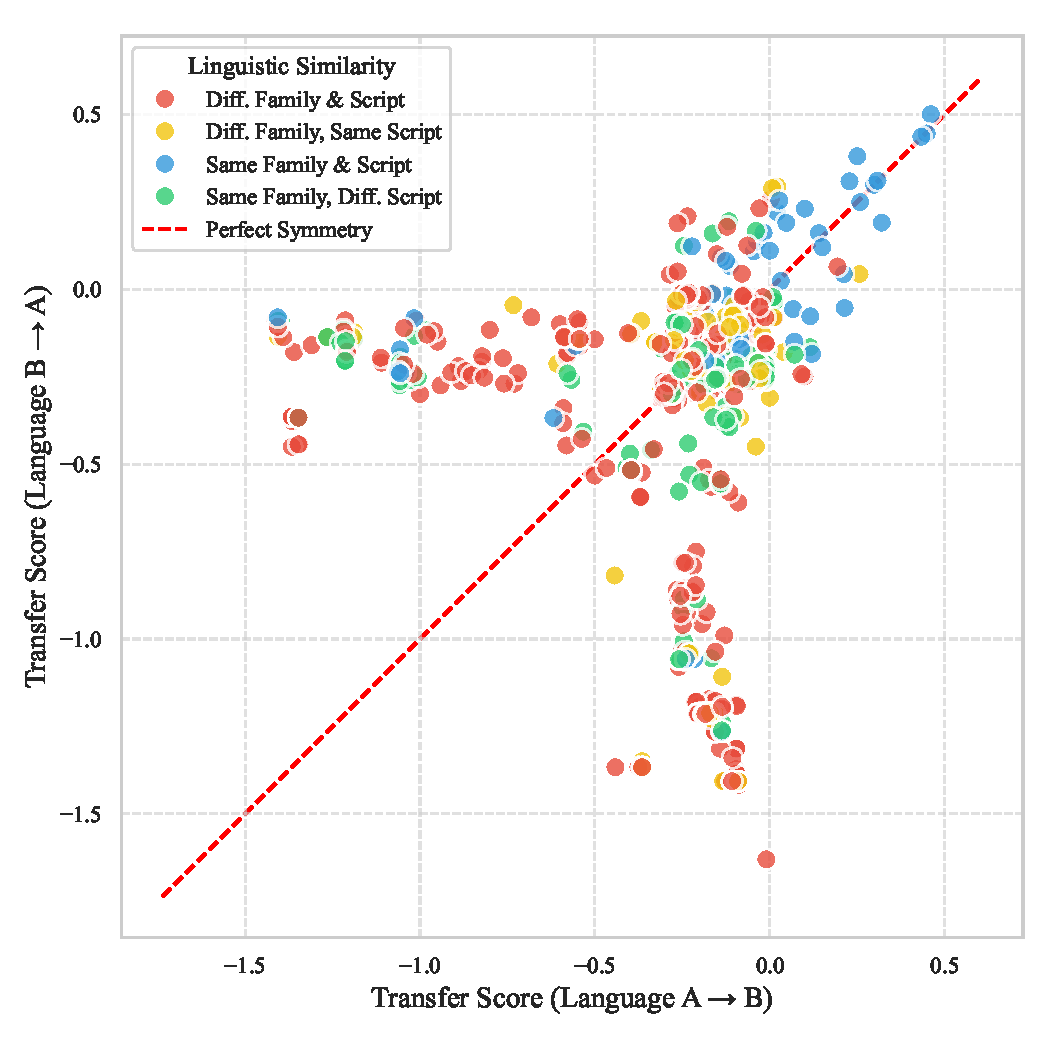
\includegraphics[width=\textwidth]{figures/language-transfer/symmetry_analysis.pdf}
        % \caption{Symmetry of language transfer, comparing the score from language A to B against the reverse direction. Points on the diagonal red line represent perfect symmetry. Points are colored by the linguistic similarity of the pair. The plot reveals a strong trend towards symmetry, with most points clustering near the diagonal. Crucially, the coloring shows that the most synergistic and symmetric pairs (top-right quadrant) are almost exclusively those sharing both language family and script. As linguistic distance increases, pairs tend to exhibit more asymmetry and less positive transfer, reinforcing the conclusion that similarity is a strong driver of bidirectional synergy.}
        \label{fig:symmetry_analysis}
    \end{subfigure}
    \hfill
    \begin{subfigure}[b]{0.45\textwidth}
        \centering
        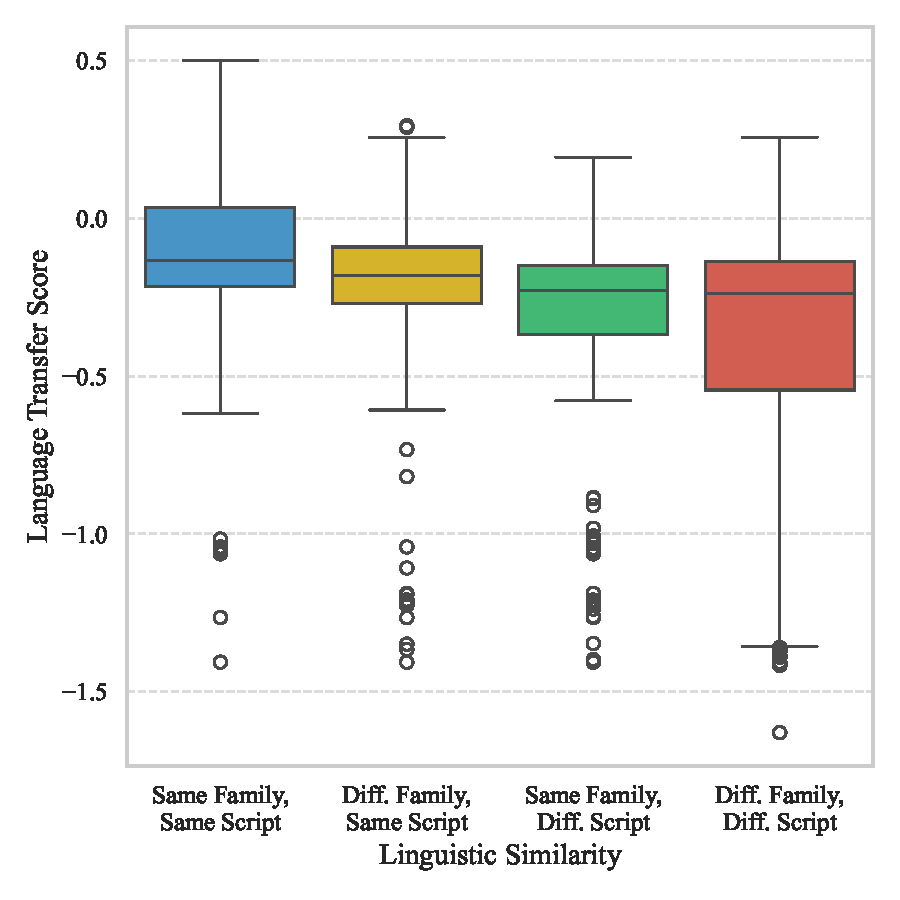
\includegraphics[width=\textwidth]{figures/language-transfer/transfer_analysis_standalone.pdf}
        % \caption{The impact of linguistic similarity on language transfer scores. The four categories of language pairs are ordered by their mean transfer score. Each box plot visualizes the distribution of scores: the central line is the median, the box spans the inter-quartile range (IQR), and the whiskers extend to $2.0\times$ the IQR. The differences between all four groups are statistically significant ($p < .001$). We find strong quantitative evidence that sharing both a language family and a script provides the greatest benefit, and that each factor independently contributes to positive cross-lingual transfer.}
        \label{fig:transfer_analysis}
    \end{subfigure}
    % \vspace{-5mm}
    \caption{\textbf{Left:} A language transfer scatter plot, comparing score symmetry: is language A as helpful to B as vice versa? Points cluster near the diagonal, indicating strong symmetry. \textbf{The most synergistic and symmetric pairs almost exclusively share both language family and script.} Greater linguistic distance correlates with increased asymmetry and reduced positive transfer.
    \textbf{Right:} The impact of linguistic similarity (via language family or script) on transfer scores. The box spans the inter-quartile range, with the median line at the center.
    \textbf{We find the differences between each group are statistically significant ($p < .001$), suggesting that sharing either a language family or a script independently contribute greater positive cross-lingual transfer.}
    }
    \label{fig:combined_analysis}
    % \vspace{-4mm}
\end{figure}

When allocating multilingual training mixtures, practitioners need to know which \emph{source} language(s) provide the most positive benefit, in co-training, to the \emph{target} language(s) they are optimizing for.
Throughout this paper, we use the terms transfer or interference to refer to the positive (or negative) inductive transfer between the training signal of two or more tasks \citep{caruana1997multitask}. 
We construct, to our knowledge, the most comprehensive matrix of language-to-language transfer scores, to assist practitioners in selecting training languages.
\[
\text{Language Transfer Score}\,\, (s \rightarrow t) = \mathrm{BTS}_{s\!\rightarrow t}  = - \frac{\sigma_{\text{bi}}(L_{\text{t}}(d_{\mathrm{mono}})) - 2d_{\mathrm{mono}}}{d_{\mathrm{mono}}}
\]
To do this, we measure how much training in a source language $s$ affects the test loss on a target language $t$. 
We define a \bts{} (\btsabb) as the relative training efficiency of a bilingual model $(s,t)=(50\%,50\%)$ compared to the monolingual model $t$ at reaching the same loss level.\footnote{We measure $\mathrm{BTS}_{s\!\rightarrow t}$ directly for $80$ language pairs, then estimate it using other training signals (with high fidelity $R^2=0.85$), as detailed in \Cref{app:lang-transfer-bts-estimation}.}
$d_{\mathrm{mono}}$ denotes a pre-defined target step (42B tokens), $L_{t}(d)$ computes the monolingual models' loss at step $d$, and $\sigma_{\text{bi}}$ finds the number of tokens for the bilingual model to reach that loss.
Because $\mathrm{BTS}_{s\!\rightarrow t}>0$ is the zero-centered, when it is $=0$ there is no transfer, $>0$ there is positive transfer, and $<0$ there is negative interference, leading to the bilingual model taking more than double the steps $d_{mono}$ the monolingual model took to reach the target loss $L_{\text{t}}(d_{\mathrm{mono}})$.
Refer to \Cref{app:language-transfer-details} for full experimental details and methodology.

In \Cref{fig:language-transfer-heatmap}, we plot the normalized \btsabb{} scores between $30 \times 30$ language pairs (or the full $38 \times 38$ in \Cref{fig:language-transfer-heatmap-full}), spanning language families and scripts, on 2B parameter models.
% This is the most expansive and rigorous language transfer matrix produced, to our knowledge, and contains many compelling observations.
Where prior work has developed comprehensive resources for measuring syntactic/phonological distances between languages \citep{khan2025uriel+}, or measured transfer scores with smaller models specifically between high and low-resource languages \citep{protasov2024super}, our work offers among the most expansive and rigorous, fully-symmetric transfer matrices, to our knowledge. 
It contains many compelling observations.
For instance, as one might expect, notable positive transfer exists between related languages, such as between Spanish, Catalan, and Portuguese, or Swedish and Norwegian, or Indonesian and Malay.
The top-5 most helpful source languages to co-train with per target are highlighted, with English appearing the most (19 of 30 instances), followed by French (16 of 30), Spanish (13 of 30), and even Hebrew (11 of 30).
In other cases, low-resource languages such as Urdu or Pashto have significant negative transfer with all other languages considered. 

\textbf{Language script, followed by language family are strongly correlated with positive transfer scores.}
In \Cref{fig:combined_analysis}, we correlate the transfer scores from the full language matrix \Cref{fig:language-transfer-heatmap}. 
Our analysis confirms a clear and statistically significant link between transfer performance and the similarity of the source and target language.
Specifically, we found sharing a script or family introduced statistically significant shifts in the mean of the transfer score (always $p<.001$).
These findings corroborate \citep{he2024scaling}'s scaling laws that grouped data by language family.
% Specifically, we found that co-training with a language from the same family results in significantly better performance compared to using a language from a different family (mean score of $-0.28$ vs. $-0.38$; t-statistic=$4.55$, p=$5.7\times10^{-6}$). 
This effect is strongest for shared scripts. 
As shown in \Cref{fig:combined_analysis}, language pairs that share the same writing system (e.g. Latin) exhibit dramatically improved transfer scores compared to pairs with disparate scripts (e.g., Latin and Cyrillic), with a mean score of $-0.23$ versus $-0.39$. 
The larger effect size for script suggests that the ability to share surface-level representations and subword vocabularies is a primary mechanism for positive transfer, more so than deeper grammatical or lexical similarities alone.
In \Cref{sec:capacity} and \Cref{app:lang-transfer} we explore how $N,D$ affect language transfer.
% We find that this extent of transfer changes greatly with scaling both tokens and parameters. We further discuss this in \cref{app:lang-transfer} and in \cref{sec:capacity}.
% \textbf{Research Question:} \emph{Are the language synergies symmetric? To what extent?}

\textbf{Language transfer scores are often symmetric within the same language family and script, but surprisingly, they cannot be assumed to be reciprocal otherwise.}
Next, we examine the extent to which language transfer is symmetric, that is, whether the benefit from language A to B is correlated to that from B to A. 
As illustrated in \Cref{fig:combined_analysis} (left), we find a surprising triangle pattern, with a Pearson correlation of $r = -0.11$.
This implies two things.
First, and perhaps most importantly, across all language pairs, there is no significant correlation, and because we observe language A is helpful to language B, \emph{we cannot assume the same in reverse.}
This corroborates findings in \citet{li2025rethinking} that altruistic languages don't always yield mutual benefits.
Second, there does appear to be a clear structure to the scatter: language pairs that share family and script (blue) cluster mostly in the top right quadrant and more tightly around the identity line, whereas language pairs with differing script and family (red) are simultaneously less symmetric, and less synergistic. 
For instance, pairs (French, Spanish) and (Russian, Ukrainian) share highly symmetric transfer scores, whereas (Chinese, Farsi) and (Russian, Vietnamese) are highly asymmetric.
We hope these findings, as well as the \Cref{fig:language-transfer-heatmap} transfer matrix, will be directly applicable to practitioners selecting language mixtures based on empirical measurements, rather than intuition.

% Most language pairs cluster tightly around the identity line, indicating a strong bidirectional relationship. This visual trend is supported by a high Pearson correlation of $r = -0.11$ between forward and reverse transfer scores. However, the analysis also highlights key asymmetries. For instance, transfer from English to many other languages is often more beneficial than the reverse, likely due to the high-resource nature of English in the pre-training data. Other pairs, such as zh-vi or zh-fa, also exhibit a significant directional preference. This suggests that while linguistic proximity creates a strong foundation for symmetric transfer, factors such as data quantity, quality, and typological divergence can introduce significant asymmetries.

% \begin{figure}[h]
%     \centering
%     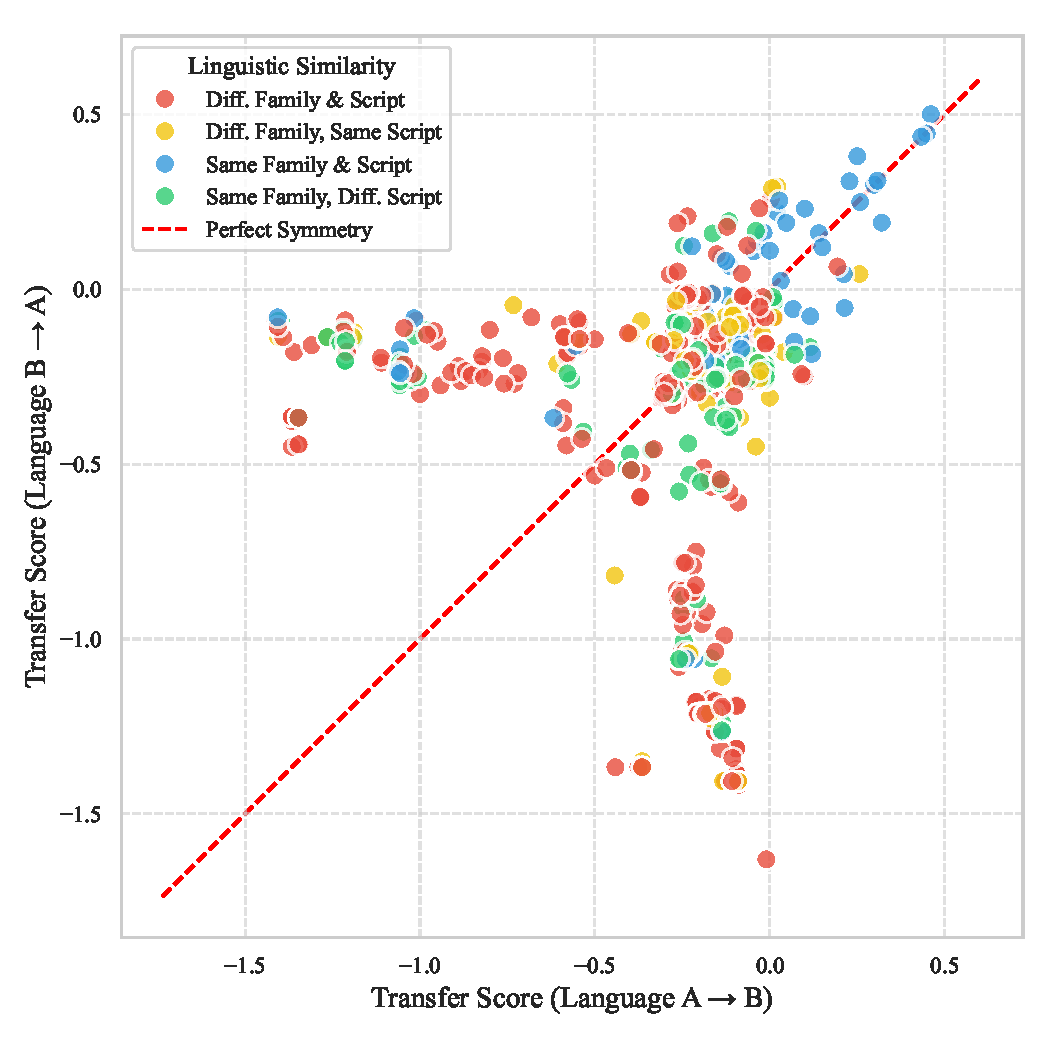
\includegraphics[width=0.5\textwidth]{figures/language-transfer/symmetry_analysis.pdf}
%     \caption{Symmetry of language transfer, comparing the score from language A to B against the reverse direction. Points on the diagonal red line represent perfect symmetry. Points are colored by the linguistic similarity of the pair. The plot reveals a strong trend towards symmetry, with most points clustering near the diagonal. Crucially, the coloring shows that the most synergistic and symmetric pairs (top-right quadrant) are almost exclusively those sharing both language family and script. As linguistic distance increases, pairs tend to exhibit more asymmetry and less positive transfer, reinforcing the conclusion that similarity is a strong driver of bidirectional synergy.}
%     \label{fig:symmetry_analysis}
% \end{figure}

% \tldr{Do language synergies appear to be based on language families or on language scripts?}

% \sayna{: the following is added to answer the above question (Do language synergies appear to be based on language families or on language scripts?). Feel free to edit.}

% To test the hypothesis that linguistic proximity drives transfer, we correlated our transfer scores from the full language heatmap (\Cref{fig:language-transfer-heatmap}). Our analysis, visualized in \Cref{fig:transfer_analysis}, confirms a clear and statistically significant link between transfer performance and the similarity of the source and target languages. Specifically, we found that co-training with a language from the same family results in significantly better performance compared to using a language from a different family (mean score of $-0.28$ vs. $-0.38$; t-statistic=$4.55$, p=$5.7\times10^{-6}$). This effect is even stronger for script similarity. As shown in \Cref{fig:transfer_analysis}b, language pairs that share the same writing system (e.g. Latin) exhibit dramatically improved transfer scores compared to pairs with disparate scripts (e.g., Latin and Cyrillic), with a mean score of $-0.23$ versus $-0.39$ (t-statistic=$7.05$, $p=2.8\times10^{-12}$). The larger effect size for script suggests that the ability to share surface-level representations and subword vocabularies is a primary mechanism for positive transfer, more so than deeper grammatical or lexical similarities captured by language family alone.


% It has been empirically observed that due to language similarities \citep{kudugunta2019investigating}, co-training similar languages can result in transfer learning between languages to result in overall better language models \citep{aharoni2019massively}. However, co-training dissimilar languages on models that are too small can result in interference, or worse performance on both languages. We seek to quantify this relationship at varying scales.

% In Figure \ref{fig:lang2lang}, we train several pairs of languages (source language X and target language Y) together with a $1:1$ sampling ratio for 40k steps, and visualize the number of steps (not total steps) needed for language Y to reach the same loss it would reach if trained alone on 10k steps. The ranges vary wildly.  We observe that some language pairs, like Spanish (es) and Portuguese (pt) require fewer than 20k steps to reach the loss achieved by training for 10k on only the target language.
% This suggests that there is positive transfer, as less than a full 10k steps of data in the target language were required to reach the desired loss.
% For language pairs that take significantly more than 20k steps to reach the target loss at 10k monolingual steps, this suggests the source language provides destructive interference.